\documentclass[12pt]{article}
\usepackage{0protoposal}
\renewcommand\contentsname{Contents\\}

\begin{document}
\begin{titlepage}
    \begin{center}
        \Large Dissertation Proposal\\for\\
        \LARGE \textsc{Peripheral Play Peculiarities}\\
    \end{center}
    \vfill
    \begin{figure}[h!]\centering
        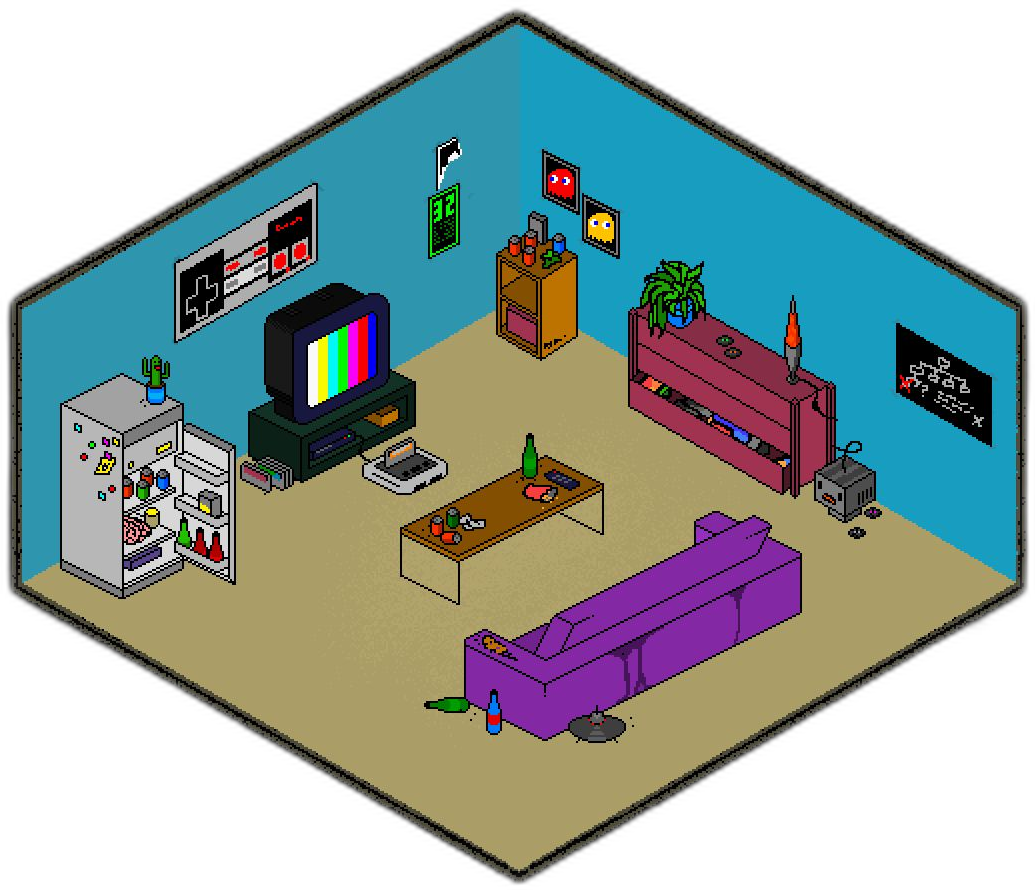
\includegraphics[width=0.6\linewidth, decodearray={0.32 1 0.32 1 0.32 1}]{game-room.png}
    \end{figure}\nocite{dsonyy}
    \vfill\tableofcontents
\end{titlepage}
\clearpage\newgeometry{left=1in, right=2cm, top=2cm, bottom=2cm}

\section{Topic of Investigation}\wordCount{450}{500}
\reversemarginpar\marginnote{\footnotesize\textsc{Keywords:}
    \textit{aesthetics, authenticity, experience, immersion, materiality, metagaming, nostalgia, paraphernalia, paratext, preservation, retrospective, transmedia}}[4cm]
\begin{abstract}\centering
    My topic of interest lies at the intersection of paratextual, corporeal, and sociocultural aspects of iconic game titles and their impact on the industry’s history.
    Paratext consists of surrounding media not included in the game itself but strongly influencing how the experience is accessed, framed, and understood.
    Material comprises the physical means and contexts of play, in turn shaping the experience through sensory input, physical feedback, and presence. 
    Society and culture permeate the above two aspects: while paratextuality is encoded in media and materiality is embedded in technology, the sociocultural layer is embodied by players themselves through their shared habits, beliefs, and informal systems.
    The co-operation of this trinity is flavoured by the aesthetics of the game playing experience in its entirety. 
    \par My project poses the following question:\vspace{2mm}
    \textbf{\textit{\\In what ways can contemporary game design achieve holistic aesthetic experiences in the likeness of iconic, historically acclaimed game titles?}}\vspace{2mm}\par 
    The research perspective is mostly aimed at context awareness and experiential revision, although, nostalgia remains a latent yet potent factor that bears investigation.
    Retrospective settings are being highlighted because most well-known titles from the past represent history as written by the victors.\footnote{Or, in a few amusingly infamous cases, the kitschy underdogs and dark horses that are often both cautionary tales and subjects of cult following. Evidently, if one struggles to attain immortality via glory, becoming an anecdote remains a viable alternative.}
    With this in mind, I believe that game design can notably benefit from closely examining the external circumstances which frame any media product's release.\par
    The theoretical research will examine existing frameworks established in game and media fields of study, intending to touch on fields and concepts such as 
    experiential aesthetics, affect theory, procedural rhetoric, immersion, metagaming, preservation, and various design approaches.
    The practical review will survey an assortment of games whose play experience is notably characterised by contextual circumstances.
    This investigation is meant to derive patterns from exemplary case studies that can suggest ways of implanting the external layers of play experience into a new piece of playable media.
    With historical awareness providing the background, some of the findings will be incorporated into designing a digital artifact complementing the written one, accompanied by fictional context in the shape of lore and paraphernalia.\par
    Comprehensive analysis of multiple real world scenarios is to be followed by a selection of applicable
    \footnote{A word which here means \parencite{asoue} "feasible".} approaches, which in turn will inform the directions taken throughout the design and development process.
    Concurrently, any relevant observations should be recorded with the intent to feed back into the writing and, eventually, provide a strong basis for reflection.
    Exercising theory in practice is expected to direct the unfolding of the game's design.
    The goal that I aspire to achieve with this project is tracing a model of media creation that is elevated by its surrounding context, and also aligns with key values established in my personal game design philosophy \parencite*[GD5609,][]{myDesignPhil}, then put the resulting framework into future practice.
\end{abstract}
\normalmarginpar\restoregeometry


\section{Survey of Sources}\wordCount{960}{1500}
    \todo[add]{Why is the research being undertaken? because vibes!}
\begin{figure}[ht]\centering
    \begin{tikzpicture}[node distance=32mm]
    % Central node
    \node (play) [pTile] {\textsc{Play}};
    % Radius of the circle
    \def\radius{32mm}
    % Peripheral nodes in circular layout
    \node (paratxt) [pTile, above of=play] {\textsc{Paratextuality}};
    \node (physics) [pTile, below of=play, xshift=-36mm, yshift=12mm] {\textsc{Physicality}};
    \node (popular) [pTile, below of=play, xshift= 36mm, yshift=12mm] {\textsc{Popularity}};
    % Connections to central node
    \draw [very thin, >=triangle 45, <->] (play) -- (paratxt);
    \draw [very thin, >=triangle 45, <->] (play) -- (physics);
    \draw [thin, >=triangle 45, <->] (play) -- (popular);
    % Dotted lines and labels
    \path [dotted, very thick] (paratxt) edge[bend right] node[midway, left]  {\small\textit{paraphernalia}} (physics);
    %\draw [dotted,thick](paratxt)--(popular)node[midway,right,xshift=4mm,yshift=-4mm]{\small\textit{or proliferation?}};
    \path [dotted, very thick] (paratxt) edge[bend left] node[midway, right]  {\small\textit{personalization}} (popular);
    \path [dotted, very thick] (physics) edge[bend right] node[midway, below] {\small\textit{preservation}} (popular);
    % Circular dashed periphery
    \draw [violet, thick, dashed] (play) circle (16mm);
    %\node (play) [left, gray, xshift=8mm, yshift=-2cm] {\footnotesize\textit{periphery}};
    \begin{scope}[transform canvas={xscale=-1,yscale=-1}]
        \path[decorate,decoration={text along path, text={perimeter},text align=center}] (1.78,0) arc[start angle=0,end angle=-300,radius=1.78];
        \path[decorate,decoration={text along path, text={perimeter},text align=center}] (1.78,0) arc[start angle=0, end angle=-70,radius=1.78];
        \path[decorate,decoration={text along path, text={perimeter},text align=center}] (1.88,0) arc[start angle=0, end angle=180,radius=1.88];
    \end{scope}
    \end{tikzpicture}
\caption{Peripheral aspects of play outside the magic circle's perimeter}
\end{figure} 

\subsection{Literature Review}
\begin{description}    
    \item[Paratextuality, a.k.a. Supporting Context]
        The initial concept by G\'{e}rard Genette \parencite*{genette} has been considerably expanded to better fit the field of game studies \parencite{consalvo}, and as a result has been entangled with adjacent terms from the original scholar's typology.
        \footnote{The five aspects of \textit{trans}textuality are \textit{inter}-, \textit{meta}-, \textit{hyper}-, \textit{archi}-, and \textit{para}-texts.}
        However, both approaches can be integrated into my own, owing to the generous overlap between the three types of external context.\par
        When strictly categorising cases, Genette's definition regards ``Elements that form a figurative threshold of a text and ground it in a socio-historical context. [...] must be created by the text’s producers or their associates".
        These can be promotional materials, introductory sequences, menus, credits, making-ofs, contextual information about authors.\par
        Meanwhile, Consalvo's interpretation covers ``Any element that forms a figurative threshold of a text and grounds it in a socio-historical context. [...] no limitations on authorship or cultural status.", akin to \textit{cultural epiphenomena}.
        This allows the inclusion of more elements like ``criticism and journalism, user discussions, fan fiction and fan art, streaming, trans-media storytelling" \parencite{svelch}.\par
        On these grounds, Genette's delineation is the more clear and straightforward directive for labelling purposes, while Consalvo's expansion on it draws a connection to cultural assimilation.
        Additionally, both have ties to materiality in their manifestation.
    \item[Physicality, a.k.a. Material Elements] \todo[add]{proper lit review}
        The most tangible of the three aspects, this refers to all the material conditions in which the game is played.
        Exclusively, this covers authentic hardware and peripherals, physical data storage, haptic features, and environmental settings.
        In addition, paratextual supplements in physical format, e.g., paper, fall under the same category to form paraphernalia.
    \item[Popularity, a.k.a. Cultural Impact] \todo[add]{proper lit review}
        Culture and society permeate the first two aspects via informal systems of shared habits, beliefs and conventions.
        The formation of social rituals by the demographic over time leads to emergent paratext, stemming from reception and circulation, and physical aspects are embodied in player presence and direct interaction with the hardware.
\end{description}

\subsection{Precedent Review}\label{sec22}
Upon stepping out of secondary academic sources, a plethora of real world situations present themselves as use case candidates.
Each listed item listed regards contemporaneous circumstances like demographic situations, business models of companies, and the technologies (both physical and software products) available, all of which steered the creative and commercial development of game titles.

While it is not imperative to audit them all individuality, I would like to present here the aspects of paratextual, material, and cultural enrichments that were pivotal to their elevation.
    
\paragraph{Pong}\phantom{.}\\
    This entry also encompasses early arcade video games and first generation home consoles line-up, with Pong \parencite{pong1972} as the paragon title.
    Their appeal lies beyond squares bouncing off rectangles, and is rooted in the outset of screen interactivity.
\begin{multicols}{3}
    \textsc{Paratextuality}\phantom{.}\\
    It predates standard paratextual materials, but it could be said that the debut of load-bearing elements, like cabinet art, operator manuals, and arcade configurations, elegantly set a precedent.
    \columnbreak\par\textsc{Physicality}\phantom{.}\\
    Physical context in the original arcade cabinets was already embodied in the requirement to be present, but the tactile precision of rotary analogue dials allowed the players to feel rooted into a simulation of a real-life table tennis match.
    \columnbreak\par\textsc{Popularity}\\
    It allowed for the onset of spectatorship. The customers of Andy Capp's Tavern had no way of knowing that this novelty would eventually by canonised as the catalyst of early video game industry. They simplywatched others compete while waiting for their own turn Way before its historical recognition, Pong simply offered a tangible shared experience, in the right place, at the right time.
\end{multicols}

\paragraph{Textual Tradition}
\subparagraph{Type-in Software}\phantom{.}
\begin{multicols}{3}
    \textsc{Paratextuality}\phantom{.}\\
    The code page is an actual part of the game, that the player inputs as the first act of participation.
\columnbreak\par\textsc{Physicality}\phantom{.}\\
    \todo[add]{Typing games into existence, bridging analogue and digital;
        machine -\> paper -\> machine;
        One typo could break everything - it was a fragile and tactile, but owned.
        Player involvement in creating or modifying the game, physical-digital bridge.}
\columnbreak\par\textsc{Popularity}\phantom{.}\\
    \todo[add]{
        learning some coding by necessity, Users often learned about BASIC or machine code doing this.;
        Engagement \& DIY Culture - Encourages direct involvement in creating or modifying the game.
    }
\end{multicols}

\subparagraph{Infocom}\phantom{.}\\ 
        Distributed \textit{feelies} for text adventures like like \textit{Zork I} \parencite*{zork1980} and \textit{Suspended: A Cryogenic Nightmare} \parencite*{suspended1983}
\begin{multicols}{2}
    \textsc{Paratextuality and Physicality}\phantom{.}\\
    In this case, the two are tightly intertwined by design. The materials were gameplay elemets integrated \textit{outside} the digital scope of the games feturing them.
\columnbreak\par\textsc{Popularity}\phantom{.}\\
    The various goodies showed alternative ways of engagement as one of the early examples of trans-media storytelling.
\end{multicols}
\todo[add]{Inscryption}

\subparagraph{MUDs and early MMOs}\parencite{mud1978}
\begin{multicols}{3}
    \textsc{Paratextuality}\phantom{.}\\
    \todo[add]{extra content\\
        Text-based, often running on university servers or via dial-up.
    } 
\columnbreak
    \textsc{Physicality}\phantom{.}\\
    \todo[add]{physical stuff\\
        The gameplay revolved around shared narrative construction, community building, and player-driven worlds.
        Early MMOs like Ultima Online and EverQuest expanded this to graphical, persistent worlds with social rituals, economies, and emergent storytelling.\\
        The sense of presence emerged through text or simple graphics combined with imagination.
        Demands of tech and scheduling affected play rhythms.
    } 
\columnbreak
    \textsc{Popularity}\phantom{.}\\
    \todo[add]{social rituals\\Immersion in world and identity building in persistent online spaces
        Social virtual worlds and emergent identity creation and online community dynamics.
        Social Spaces as Core Feature
        Players were often co-creators, shaping lore, communities, and even rules.
        Community dynamics formed the metagame with the rise of player politics, guilds, and conventions.
        Nostalgia \& Cultural Memory - Early MUDs are often remembered fondly as social spaces beside games.
    }
\end{multicols}

\paragraph{Transmedia Storytelling}
\subparagraph{Swordquest}
Atari's Swordquest contest extended gameplay beyond screens to the real world by mixing physical and digital elements:
    \begin{enumerate}
        \item Earthworld \parencite*{swordquest_earthworld1982} introduced the series' puzzle-driven model, integrating comics, game mechanics, and a real-world treasure hunt for a solid gold talisman; launched with a DC Comic tie-in and puzzle contest
        \item Fireworld \parencite*{swordquest_fireworld1983} leaned further into cryptic puzzle design and real-world participation. Its solution required synthesizing symbolic logic from in-game events and comic references; continued the trans-media puzzle format with a new comic and prize quest
        \item Waterworld \parencite*{swordquest_waterworld1983} was the (unintentionally) final released in limited numbers, making it a rare case of high-concept interactive media collapsing due to external economic factors (the 1983 crash) - a cautionary historical moment; prize was still awarded though
    \end{enumerate}
\begin{multicols}{3}
    \textsc{Paratextuality}\phantom{.}\\ \todo[add]{extra content} \columnbreak
    \textsc{Physicality}\phantom{.}\\ \todo[add]{physical stuff} \columnbreak
    \textsc{Popularity}\phantom{.}\\ \todo[add]{social rituals}
\end{multicols}
\subparagraph{AR Games}\cite{sicart-argo}
\todo[add]{ARGs like Frog Fractions 2 or Pokémon GO - real-world participation, secrecy, and communal knowledge.}

\paragraph{Curated Retro Compilations}
\subparagraph{Digital Eclipse}\phantom{.}\\
Their efforts in authentic and curatorial preservation are evident in \citetitle{atari50}, \citetitle{tmnt2022}, and even more so in their \textit{Gold Series} of interactive documentaries, starting with \citetitle{karateka2023} and including \citetitle{llamasoft2024} and \citetitle{tetris2024}.
\begin{multicols}{2}
    \textsc{Paratextuality and Physicality}\phantom{.}\\ 
    \todo[add]{Interactive timeline museums where physical paratext is digitised; Archival materials (concept art, pitch documents, developer commentary) as interactive content.} 
    \columnbreak\textsc{Popularity}\phantom{.}\\ \todo[add]{Metagame - play the in-the-moment cultural context.}
\end{multicols}
\subparagraph{Sega Genesis Classics}\parencite{sega_classics}
    \todo[add]{Compare approach with DE: education vs. nostalgia}
\begin{multicols}{3}
    \textsc{Paratextuality}\phantom{.}\\ 
    \todo[add]{Aesthetic vs. archival: It simulates the feel, not the making-of. No material outside the bedroom} 
    \columnbreak\textsc{Physicality}\phantom{.}\\ 
    \todo[add]{Replicate childhood gaming by framing ROMs within a stylised memory space.; Nostalgia Theatre: A 1990s bedroom with a CRT TV, a shelf of cartridges, and other dressing like posters, lava lamps, beanbags}
    \columnbreak\textsc{Popularity}\phantom{.}\\ 
    \todo[add]{Theatricality vs. Fidelity: It romanticises the idea of an era}
\end{multicols}

\paragraph{Foundational NES Titles}
\subparagraph{Dragon Quest I}\parencite{dragonquest1986}
    \todo[gpt]{Early JRPG with lots of wandering, grinding, and guesswork. QoL changes in remasters remove friction.
        Friedrich Kittler emphasizes how media technology determines UX - NES constraints + JRPG design = a new literacy.
        Questions:
            What is left of a game's intended experience once its context is stripped away?
            Can design elements once seen as "limitations" be re-evaluated as experiential depth?
            How did early JRPGs rely on extra-diegetic tools (manuals, maps, player-created notes)?}
\begin{multicols}{3}
    \textsc{Paratextuality}\phantom{.}\\\todo[add]{Original JP release had a detailed manual with monster illustrations, hints, lore, and walkthroughss; later titles also saw promotional manga and other media support.} \columnbreak
    \textsc{Physicality}\phantom{.}\\\todo[add]{lengthy play sessions, manual-driven mechanics; manual notation of maps, quests, and clues. box art, manual, and cartridge were the game as much as the 8-bit world onscreen.\\Commitment shaped by hardware constraints, difficulty, as well as a contrived saving system in the JP version.} \columnbreak
    \textsc{Popularity}\phantom{.}\\\todo[add]{Cultural Moment	In Japan, it was released into an infant console gaming culture.\\The response helped shape how audiences engaged with fantasy and how RPGs developed worldwide.
}
\end{multicols}

\subparagraph{Legend of Zelda}\parencite{zelda1986}
\begin{multicols}{3}
    \textsc{Paratextuality}\phantom{.}\\ \todo[add]{Manuals, gudes, Nintendo Power} \columnbreak
    \textsc{Physicality}\phantom{.}\\ \todo[add]{Manuals, gudes, Nintendo Power, mapping} \columnbreak
    \textsc{Popularity}\phantom{.}\\ \todo[add]{extrenal collaboration, knowldge sharing as a social currency?}
\end{multicols}
\todo[add]{Tunic}

\subparagraph{Startropics}\parencite{startropics1990}
\begin{multicols}{3}
    \textsc{Paratextuality}\phantom{.}\\ \todo[add]{Serves as a mechanic; like Infocom's feelies, it's between fundamental and supplemental } \columnbreak
    \textsc{Physicality}\phantom{.}\\ \todo[add]{External Narrative Elements requiring real-world interaction to progress; A letter packed with the game needed to be dipped in water to reveal a secret code (747).} \columnbreak
    \textsc{Popularity}\phantom{.}\\ \todo[add]{Consequences of removing/simulating physical components in digital re-releases; Nintendo hotline trends; }
\end{multicols}

\paragraph{Mario Paint}\parencite{mariopaint1992}
\begin{multicols}{3}
    \textsc{Paratextuality}\phantom{.}\\ \todo[add]{extra content} \columnbreak
    \textsc{Physicality}\phantom{.}\\
    The SNES mouse peripheral introduced a creative method of interaction.
\columnbreak
    \textsc{Popularity}\phantom{.}\\ \todo[add]{social rituals}
\end{multicols}
\todo[ref, inline]{Legacy in Ring Fit Adventure and Nintendo Labo}

\paragraph{Dragon's Lair}\parencite{dragonslair1983}
    \todo[add]{Immersive Presentation: A case of experiential obsolescence and preservation challenges. }
\begin{multicols}{3}
    \textsc{Paratextuality}\phantom{.}\\
    \todo[add]{Context-Dependent Play} 
\columnbreak
    \textsc{Physicality}\phantom{.}\\
    \todo[add]{The fragility of experience tied to hardware \& setting} 
\columnbreak
    \textsc{Popularity}\phantom{.}\\
    The quality of the gameplay experience is entirely dependant on the setting in which it is attempted (that is to say it is relatively obsolete now, though significantly influential for its time)
\end{multicols}
\todo[ref, inline]{Mention VR titles like Half-Life: Alyx.}

\paragraph{Doom}\parencite{doom1993}
    \todo[gpt]{Technical breakthrough and modding culture shaping player agency and community.
                Relevance: A milestone in tech-driven immersion, multiplayer, and player-created content.
            Unique Focus: Emphasizes shareware distribution, modding culture, and emergent multiplayer experiences.
            Distinguishes itself by: Showcasing technology's role in shaping community and cultural phenomena.
        1. Technical Breakthrough \& Experiential Leap
            Doom was revolutionary for bringing fast-paced, immersive 3D-like gameplay to home computers.
            It ran on widely available hardware, but pushed boundaries - allowing players to feel like they were "inside" a game world for the first time.
            The networked multiplayer aspect introduced new social dynamics (death-matches, co-op).
            The experience was the rush of playing something new, fluid, intense.
        2. Distribution \& Modding Culture
            Doom popularized shareware distribution.
            This facilitated the early modding scene, where players created and shared WADs.
            Game's "life" was extended beyond the original release.
            Its materiality is an ecosystem of player-generated content, forums, and zines.
        How Doom Fits Your Themes
            Physicality of Play	Hardware choices and physical setup influenced play intensity and social gatherings (LAN parties).
            Meta Gaming	Doom's modding community exemplifies metagaming as an extension of play and cultural relevance.
        Questions
            How did Doom's novel tech and shareware model redefine the player's relationship with games and communities?
            In what ways did physical hardware and social context enhance or limit the "original" Doom experience?
            How does the modding culture around Doom reflect early forms of metagaming and participatory culture?}
\begin{multicols}{3}
    \textsc{Paratextuality}\phantom{.}\\ \todo[add]{extra content} \columnbreak
    \textsc{Physicality}\phantom{.}\\ \todo[add]{physical stuff} \columnbreak
    \textsc{Popularity}\phantom{.}\\ \todo[add]{social rituals}
\end{multicols}

\paragraph{Celebrations of Circumstances}
\subparagraph{Feature Phone Mobile Games (J2ME/BREE era) Boom in Japan}\phantom{.}
    \todo[gpt]{Ubiquitous handheld play integrated into daily life rhythms; mobile gaming scene before smartphones
            Gaming on-the-go, often during commutes or small pockets of free time.
            Temporal, spatial, and ergonomic constraints.
        1. Environment Driven Design - tailored to short bursts, played standing up in trains or waiting at stations.
            Navigation designed for T9 input, small screens, and no touch; clarity and feedback prioritised over sound
        2. Networked Paratext
            Many of these were subscription-based, offered via carrier portals (like i-mode by NTT Docomo).
            Games were part of an ecosystem of ringtones, wallpapers, manga, and communication tools.
            Part of a wider lifestyle aesthetic.
        3. Transience and Cultural Memory
            These games often weren't preserved, and emulating them is notoriously difficult.
            Yet they were formative for a whole generation - influencing everything from gacha mechanics to asynchronous multiplayer.
            They became folk games of a sort: shared, modified, talked about more than archived.
        Theory
            Metagaming  The ecosystem (portal + phone + community) is the game.
            McLuhan - The medium is the message	The form factor (commuter phone) shaped behaviors and design logic.
            Miyazaki's Ludic Nostalgia (????)
            Does this era reflect a Japanese-specific yearning for transient, everyday magic - gaming anonymously amid others?
        Question: Can games built for transient or ephemeral contexts still produce deep emotional resonance?}
\begin{multicols}{3}
    \textsc{Paratextuality}\phantom{.}\\ \todo[add]{extra content} \columnbreak
    \textsc{Physicality}\phantom{.}\\ \todo[add]{physical stuff} \columnbreak
    \textsc{Popularity}\phantom{.}\\ \todo[add]{social rituals}
\end{multicols}
\todo[ref, inline]{Dragon Quest i-mode remakes - stripped-down, episodic versions designed for 10-minute sessions.
            RPGs like Elminage or Wizardry Gaiden .
            Konami's i-appli ports of classic games, reinterpreted for d-pad and one-handed controls.}
\subparagraph{Cosy COVID}\cite{acnh2020}
    \todo[add]{Comfort games as safe spaces during historical moment of crisis; slow, reflective, and socially connective play; Environment and UI (simple tools, gentle music, slow pace) tuned to match a collective emotional state}
\begin{multicols}{3}
    \textsc{Paratextuality}\phantom{.}\\ \todo[add]{Paratextual ecosystem (memes, tutorials, fan guides, in-game design templates) } \columnbreak
    \textsc{Physicality}\phantom{.}\\ \todo[add]{physical stuff} \columnbreak
    \textsc{Popularity}\phantom{.}\\ \todo[add]{Launched days after global lockdowns began
            Filled the social void through visiting friends' islands
            Gained traction as a shared, ritualised, soothing routine
            People made birthday parties, weddings, protests, in-game markets, art installations and fashion shows
            emergent social value and community-building.
        Physical/social context (quarantine, anxiety, disconnection) gaving meaning}
\end{multicols}
    \todo[ref, inline]{Other titles with shared elements flourising in the same era: Stardew Valley, Spiritfarer, Among Us, Cozy Grove, Unpacking. They often feature physical-world metaphors (gardening, home decorating, friendship building); Low-stress, high-emotion mechanics; Emphasis on customisation, routine, and community}

    \todo[ref, inline]{Include UFO50, Tunic, Outer Wilds, Hypnospace Outlaw}
    \todo[add]{Peripherals: Light Gun, Labo, Ring Fit for embodied play}
\newpage


\section{Methodology}\wordCount{34}{200}     
In order to tackle the research question, the following methods are under consideration:
\begin{description}
    \item[Textual, ludic and comparative analyses and syntheses]
        Will be used for scholarly research, deconstructing key game precedents, and formulating the main thesis.
    \item[Theoretical framework conceptualisation and application]\todo[add]{Triple P}
    \item[Research through design (RtD)]\todo[add]{What does it mean?}\todo[ref]{source}
    \item[Media archaeology and (maybe) reception studies]\todo[add]{hardware, display fidelity, manual paraphernalia}
    \item[Autoethnography]\todo[add]{to test claims}
\end{description}
\newpage


z
\begin{figure}[ht]\centering    
    \begin{tabular}{l | r} Essay Writing & Game Prototype                           \\\hline
        \textcolor{chap0}{\textit{Proposal} document and review}               
        &\textcolor{chap0}{Initial concept ideation in a paragraph}                 \\\hline
        \textcolor{chap1}{\textit{Introduction}, \textit{Literature Review}},  
        &\textcolor{chap1}{Design document outlining concept and specs}     \\
        \textcolor{chap1}{and \textit{Case Studies} chapters}                  
        &\textcolor{chap1}{to be used as the first piece of supplemental material} \\\hline
        \textcolor{chap2}{\textit{Research through Design} chapter}            
        &\textcolor{chap3}{Vertical/Proof-of-Concept build; manual booklet draft}   \\\hline
        \textcolor{chap3}{\textit{Synthesis} and \textit{Conclusion} chapters} 
        &\textcolor{chap3}{Playable game, guide and/or magazine page drafts}        \\\hline
        \textcolor{chap4}{Editing and finalising writing}                      
        &\textcolor{chap4}{Late stage game development; finalising paraphernalia}
    \end{tabular}   
    \caption{Above: Progress stages to complete in parallel:
        \\Below:Project pipeline with progress milestones, dates are subject to change}\vspace{8mm}
            
    \begin{tikzpicture}
        [% Better alignment, see https://tex.stackexchange.com/questions/315075
            every node/.style={font=\scriptsize, text height=1ex, text depth=.25ex}
        ]
        % horizontal time line   
        \draw[-] (0,0) -- (16,0);
        % draw vertical lines
        \foreach \x in {0.17,0.34,...,15.64} { \draw[color=lightgray] (\x cm,-2pt) -- (\x cm, 2pt); } % days
        \foreach \x in {1,2,...,15}          { \draw[color=gray]      (\x cm, 0pt) -- (\x cm, 4pt); } % weeks
        \foreach \x in {5.2,10.55}           { \draw                  (\x cm,-4pt) -- (\x cm, 4pt); } % months
        \draw[color=black] (10.55, 0) -- (10.55, -0.6) node[below] {2026};
        % place axis labels
        \node[anchor=north] at (2, -0.4) {November};
        \draw[color=gray] (3.45,0) -- (3.45,-0.2) node[below] {$20^{th}$};
        \node[anchor=north] at (8, -0.4) {December};
        \draw[color=gray] (7.78,0) -- (7.78,-0.2) node[below] {$15^{th}$};
        % Winter Break:             15 December - 2 January
        % Autumn Assessment Period:  5 January - 23 January
        \draw[color=chap0] (7.78, -0.2) -- (10.9, -0.2) node[midway, above, yshift=-14mm, text=chap0] {Winter Break};
        \draw[color=chapZ] (11.42,-0.2) -- (14.5, -0.2) node[midway, above, yshift=-14mm, text=chapZ] {Assessment Period};
        \node[anchor=north] at (13,-0.4) {January};
        \draw[color=gray] (10.9, 0) -- (10.9, -0.2) node[below] {$2^{nd}$};
        \draw[color=gray] (11.42, 0) -- (11.42, -0.2) node[below] {$5^{th}$};
        \draw[color=gray] (12.11, 0) -- (12.11, -0.2) node[below] {$9^{th}$};
        \draw[color=gray] (12.6, 0) -- (12.6, -0.2) node[below] {$12^{th}$};
        \draw[color=gray] (14.5, 0) -- (14.5, -0.2) node[below] {$23^{rd}$};
        % Text markers
        \draw[color=chap0,>=triangle 45 reversed, <-] (4.20,0) -- (4.20,  1) node[above, align=center, text=chap0] {Proposal\\review};
        \draw[color=chap1,>=triangle 45 reversed, <-] (5.67,0) -- (5.67,0.4) node[above, align=center, text=chap1] {First 3 chapters and a\\game design document};
        \draw[color=chap2,>=triangle 60 reversed, <-] (7.65,0) -- (7.65,1.4) node[above, align=center, text=chap3] {RtD - chapter and\\vertical prototype};
        \draw[color=chap3,>=triangle 90 reversed, <-] (11.11,0) -- (11.11,0.4) node[above, align=center, text=chap4] {Essay-written;\\artifact-presentable \\supplementals-ongoing};
        \draw[color=chap4,>=triangle 45 reversed, <-] (12.6,0) -- (12.6,  1) node[above, align=center, text=chapZ] {Submission\\deadline};
    \end{tikzpicture}
\end{figure}\vspace{-8mm}
\paragraph{Approach}As long as its laden with enough peripheral context, the practical component can be of any genre to begin with.
In essense, it must be a meta-game, which poses as either a modern piece with retro sensibilities, or a remaster of an ersatz effigy from an alternative, but not too unlike our own, reality.
Since the eventual aim of this research project is to understand how to achieve the former, perhaps the latter would be a better subject for experimentation.
    \todo[add]{Hides crucial lore in the periphery, without which it cannot be completed}
\paragraph{Elements and Features}
    \todo[add]{Manual (instructional play), guides, prompts in varied formats (e.g., real-world clues), magazine pages, reviews, developer commentary, margin notes and illustrations, ads and headlines (for flavour). Reinforcement of manual discovery, note-taking and blind exploration}
    \todo[add]{Control peripherals, printables (above)}
    \todo[add]{World-building with historical Events (or contests), Word-of-mouth rumour simulation}
\paragraph{Scope}
    \todo[add]{Differentiate between real and replicated constraints (time, skill, vs. media, software/hardware)}
    \todo[add]{Speculate on scale vs. feasibility and layer implementation plans vertically}
    
\paragraph{Technology Toolset:}
\begin{description}[noitemsep]
    \item{\textbf{\LaTeX}} is my preferred typesetting system, which I will extensively use to produce documents for both the written component and any potential paraphernalia, such as maps, guides, or manuals.
    \item{\textbf{Unity}} is the 3D game engine I am most familiar with, offering lots of versatility and good supporting documentation and teaching materials. \textsc{However}
    \item{\textbf{Godot}} is a lightweight and versatile open-source 2D and 3D game engine that I have been meaning to explore as an alternative. 
    \item{\textbf{Git}} is the version control standard, so \textbf{GitHub} will archive all documentation and source code.
\end{description}

\paragraph{Assets} will be sourced mostly from open content websites. 
\begin{itemize}[label=\faSearch, noitemsep]
    \item \texttt{itch.io}\parencite*{itchio} - the topmost provider and a favoured digital distribution platform for indie developers
    \item \texttt{kenney.nl}\parencite*{kenney} - offers various 2D and 3D asset packs that congruously fit together
    \item \texttt{quaternius.com}\parencite*{quaternius} - similarly to Kenney's, this online collection operates under a \textit{\textbf{CC0} (Creative Commons Zero) open source license}, and features a sizeable line-up of 3D assets
    \item \texttt{opengameart.org}\parencite*{opengameart} - mildly chaotic in comparison to the options listed above, but a large and long lived library for libre content
\end{itemize}
\clearpage


\section{Chapter Breakdown}\wordCount{350}{200}
\begin{description}
    \chapterplan{chap0}{Introduction}{400 words / 5\%}{\hspace*{-2em}
        Declaration of the research topic and question, their field, and relevance to game studies;\\\hspace*{-2em}
        Clarification of vocabulary such as `holistic' and `authenticity', as well as `experiential aesthetics';\\\hspace*{-2em}
        Pitch of the practical part and its connection to the writing.}
        {Contextual framing and problem definition}
        {Overview of primary and secondary titles}
        
    \chapterplan{chap1}{Literature Review}{2400 words / 30\%}{\hspace*{-2em}
        Definition of key terminology; contextualising the \textbf{P-}trinity through the secondary sources.}
        {Thematic synthesis, conceptual frameworking}
        {\srcBullet{chap1} Friedrich Adolf Kittler versus Marshall McLuhan \parencite{mcluhan} on media theory \todo[ref]{possibly optional}
            \srcBullet{chap1} \citework{svelch}
            \srcBullet{chap1} \citebook{kirschenbaum}
            \srcBullet{chap1} \citeconf{bogost-platform}
            \srcBullet{chap1} \citework{galloway}
            \srcBullet{chap1} \citebook{boluk-lemieux}
            \srcBullet{chap1} \citebook{consalvo}
            \srcBullet{chap1} \citebook{grimes}
            \srcBullet{chap1} \citework{keogh}
            \srcBullet{chap1} \citebook{gitelman}
            \srcBullet{chap1} \citebook{hjenkins} 
            \srcBullet{chap1} \citebook{taylor}
        }
    
    \chapterplan{chap2}{Case Studies}{1800 words / 22.5\%}{\hspace*{-2em}
        Framing real-life settings in the context of paratextuality, physicality, and popularity;
        \\\hspace*{-2em} Further analysis to extract practical inferences.}
    {Media archaeology, theoretical framework application, ludic and paratextual analysis, comparative synthesis}
    {A curated subset of primary sources listed in Section \ref{sec22}, along with:
        \srcBullet{chap2} \citebook{sicart-argo}
        \srcBullet{chap2} Fan-based zines and archives, e.g., Your Sinclair, Commodore User, Compute!, Antic, etc.
        \srcBullet{chap2} The Internet Archive / The Wayback Machine \parencite*{archiveorg}}
    
    \chapterplan{chap3}{Development}{1400 words / 17.5\%}{\hspace*{-2em}
        Chronicle of the RtD process and explanation how,
        \\\hspace*{-2em} in designing a prototype to interrogate a question, theory informed practice and vice versa;
        \\\hspace*{-2em} Recognition/acknowledgement of any setbacks or limitations.}
    {Research through Design, Ludic/comparative analysis}
    {Primary sources with strong parallels to my direction; plus guidance from reading:
        \srcBullet{chap3} \citebook{rusch}}
    
    \chapterplan{chap4}{Synthesis}{1600 words / 20\%}{\hspace*{-2em}
        Revision of the artifact; Discussion on theory in practice:
        \\\hspace*{-2em} how the two informed, or clashed with, each other;
        \\\hspace*{-2em} Correlation with primary sources;
        \\\hspace*{-2em} Provisional answer to the research question.}
    {Comparative ludic analysis, auto-ethnographic reflection}
    {Secondary sources that share concerns with the artifact}
    \chapterplan{chapZ}{Conclusion}{400 words / 5\%}{\hspace*{-2em}
        Reflection of what has been achieved;\\\hspace*{-2em}
        Outline of implications and further open-ended research directions to build upon.}
    {Critical reflection and projection}
    {Recommendations for reading/playing not mentioned in earlier chapters}
\end{description}
\newpage


\section{References}
\printbibliography[title={Bibliography}, nottype=software, nottype=misc, nottype=online]
\newpage\printbibliography[title={Ludography},type=software]
    \todo[ask]{'Is it mandatory to add \textbf{date played}? I don't see much value in that information:\\
        some I have played ages ago while some I have not at all but am sufficiently informed about.}
\printbibliography[title={Artefact Assets Appendix}, filter=assets]
\end{document}